%!TEX root = ../thesis.tex

\chapter{资料及模式介绍}

\section{原位观测}

\subsection{臭氧探空}

针对中国东南部的强对流天气,于2019年7月25日和2020年9月1日
在南京国家基准气候站(31.93$^{\circ}$ N,118.90$^{\circ}$ E)共释放了五个臭氧探空仪。
为了研究对流的影响,我们分别在对流发生前和对流发生中/对流发生后各释放一次探空。
深对流概况及臭氧探空仪轨迹见图\ref{fig:ozonesonde}。

\begin{figure}[H]
\centering
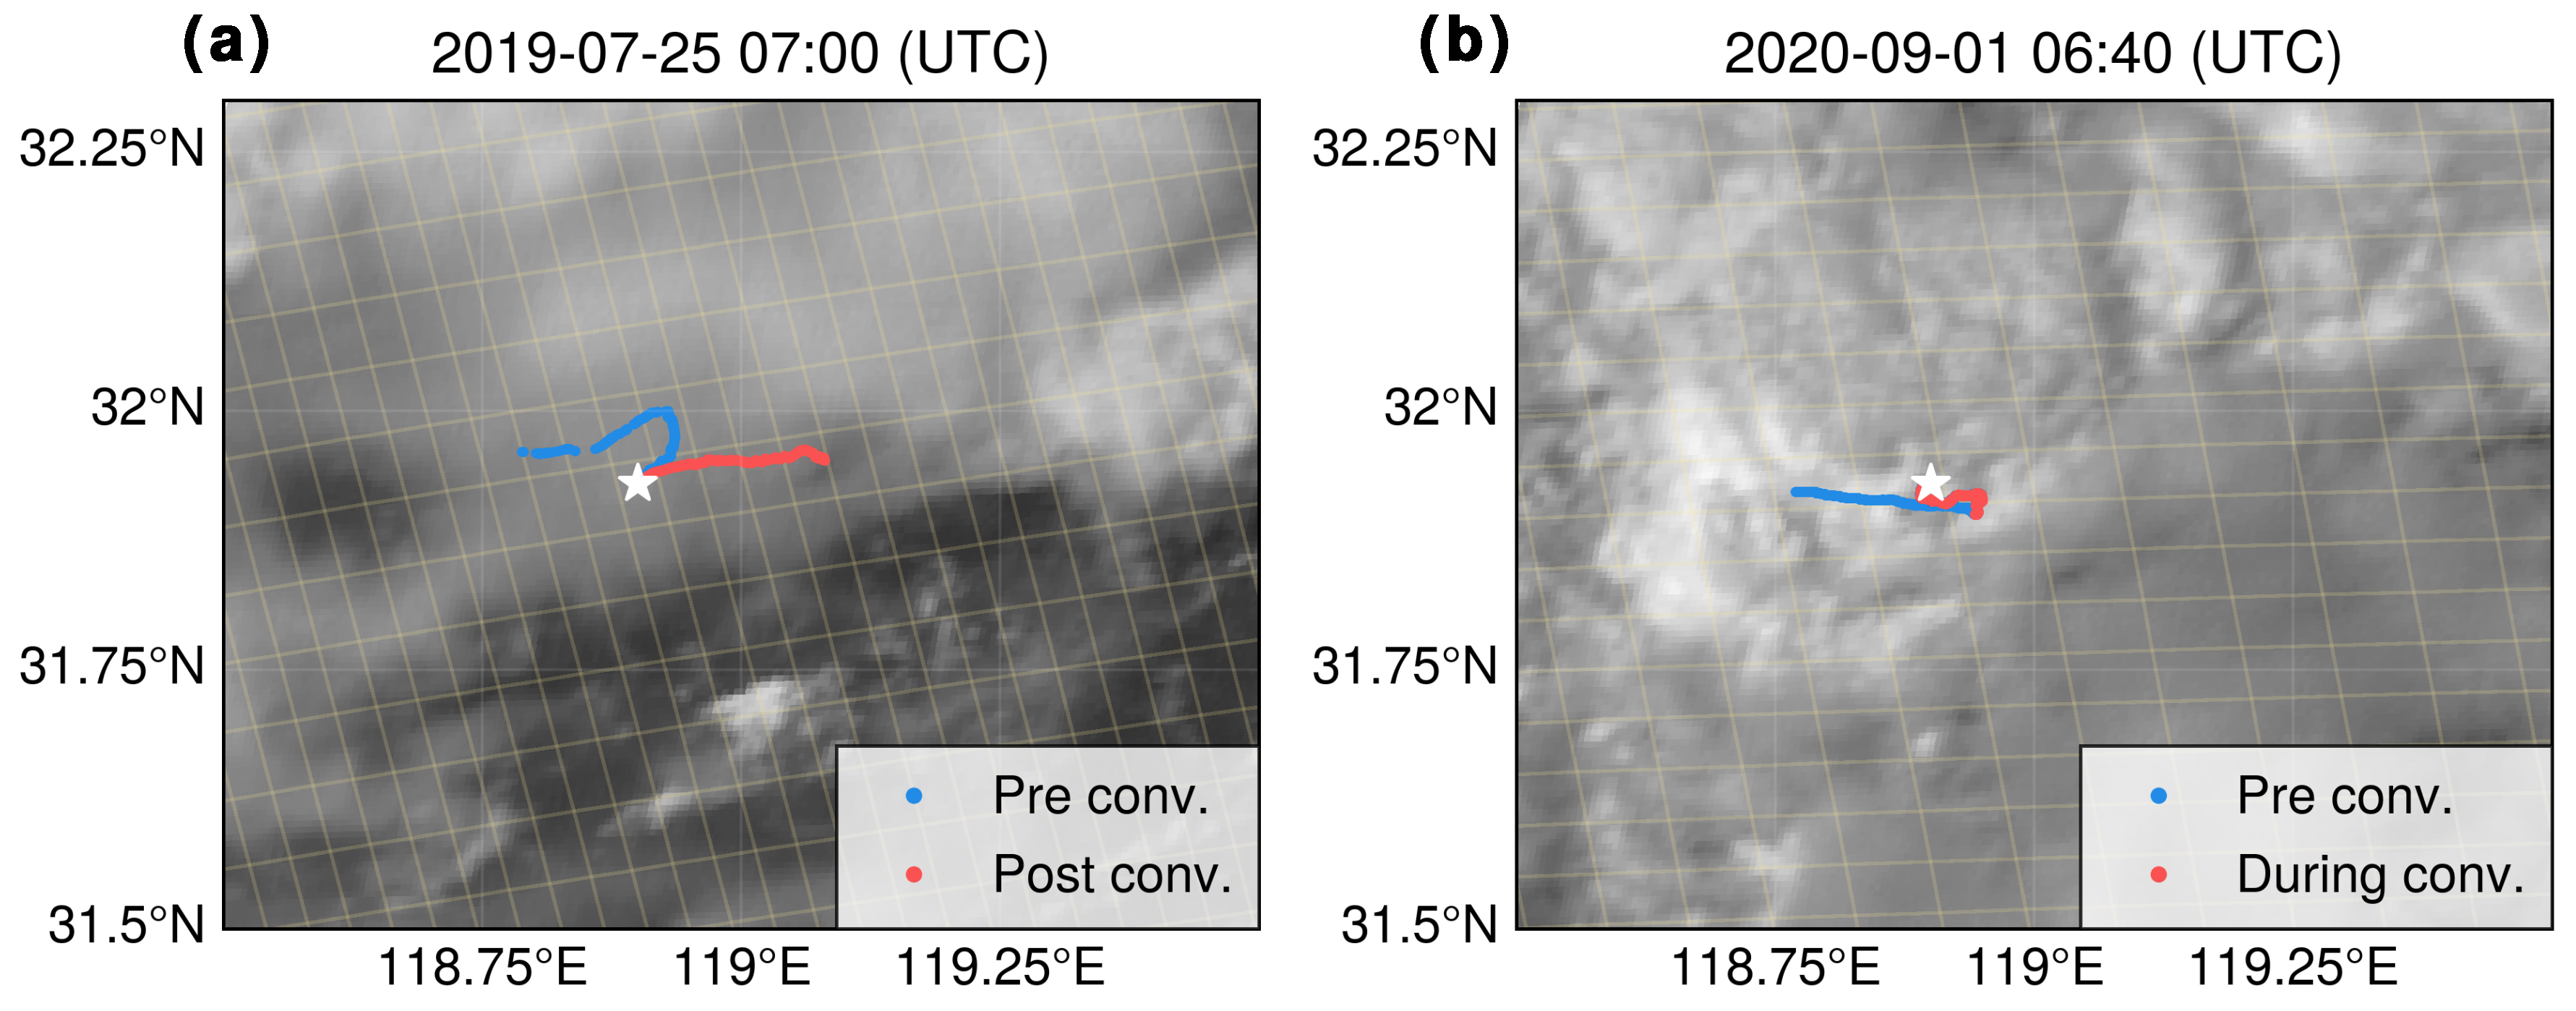
\includegraphics[width=0.9\textwidth]{./figures/ozonesonde.png}
\caption{在对流后或对流中的臭氧探空仪达到约 10 km时,风云4A先进地球静止辐射成像仪(AGRI)可见通道(0.65 $\mu$m)探测到的对流。
对流前的臭氧探空仪轨迹为蓝色,其他为红色。白星符号代表观测站,细黄线是TROPOMI像素条带。\\
Figure \ref{fig:ozonesonde}. The convection detected by the FY-4A Advanced Geostationary Radiation Imager (AGRI)
visible channel (0.65 $\mu$m) field at the time when the post-convection/during-convection ozonesondes reached around 10 km.
The pre-convection ozonesonde trajectories are colored blue while others are in red.
The white star symbol stands for the observation station and the thin yellow lines are the TROPOMI swath pixels.
}
\label{fig:ozonesonde}
\end{figure}


具体而言,2019年7月25日发生的对流为热对流,释放的三个臭氧探空均产自中国大气物理研究所(IAP)。
IAP 臭氧探空仪使用电化学浓差电池(ECC),其完整参数和性能见\citet{Zhang.2014}。
就性能而言,从地表到2.5 km平均偏差小于0.3 mPa,9 km以下接近零,9--18 km之间小于0.5 mPa。
第一台IAP臭氧探空仪于7月23日(晴天)05:35 UTC释放,另外两台分别于7月25日05:10 UTC(对流前)和06:35 UTC(对流后)释放。
由于防水故障,对流前释放的探空仪在释放后几秒钟就失去了信号,故而我们选择了7月23日释放的臭氧探空仪作为对流前的数据。
虽然时间间隔为2天,但10 km以上预报的O$_{\ch{3}}$廓线最大相对差异通常小于25\%(图\ref{fig:waccm_forcast_o3}),
因此O$_{\ch{3}}$日变化不足以解释探空观测到的超过65\%的差异。

此外,两台维萨拉(VAISALA)ECC臭氧探空仪分别于8月31日23:45 UTC(对流前)和9月1日06:10 UTC(对流期间)成功释放。
准备工作及具体操作均遵循标准手册,确保精度优于5\%,且30 km 以下的精度在$\pm$(5--10)\% 以内\citep{Smit.2007}。
该次探空试验所捕获的飑线是由冷空气和台风梅萨克(Maysak)外围环流的汇合发展而来的。
值得强调的是,对流期间的臭氧探空仪直接穿入云层,为探索受对流云影响的O$_{\ch{3}}$提供了独特的机会。

\begin{figure}[H]
\centering
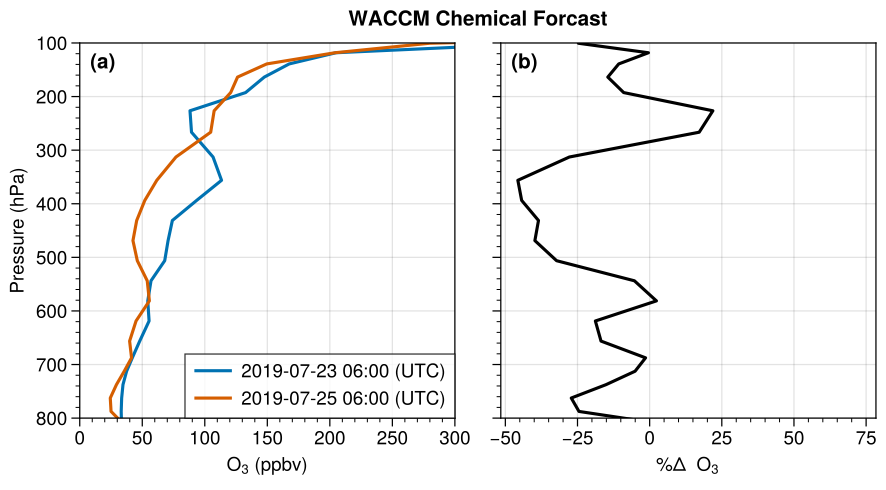
\includegraphics[width=0.9\textwidth]{./figures/waccm_forcast_o3.png}
\caption{(a)全大气层气候模型(WACCM)预报场的区域平均(118.5--119.5$^{\circ}$ E, 31.5--32.5$^{\circ}$N)O$_{\ch{3}}$廓线。
蓝色为对流前,橙色为对流后。(b)为(a)中O$_{\ch{3}}$廓线的百分比差异。\\
Figure \ref{fig:waccm_forcast_o3}. (a) Regional mean (118.5$^{\circ}$E – 119.5$^{\circ}$E, 31.5$^{\circ}$N – 32.5$^{\circ}$N)
pre-convection (blue) and post-convection (orange) O$_{\ch{3}}$ profiles from the 6-hour Whole Atmosphere Community Climate Model (WACCM) forecasts.
(b) The percent difference of O$_{\ch{3}}$ profiles in (a).
}
\label{fig:waccm_forcast_o3}
\end{figure}

\subsection{闪电数据集}

在\ref{sec:retrieval}章美国大陆的研究中,我们使用了整体闪电探测网(ENTLN)。
ENTLN运营着一个由全球1500多个地面站组成的系统,在美国大陆安装有900多个传感器\citep{Zhu.2017,Marchand.2019}。
CG和IC均由传感器根据电场脉冲极性和波形进行定位,检测频率范围为1 Hz 至 12 MHz。
如果脉冲组在700 ms和10 km范围内,它们则被归类为闪电。
在ENTLN的预处理数据中,包括了闪击和由一个或多个闪击组成的闪电。
\citet{Rudlosky.2015}将ENTLN组合事件(CG和IC)与LIS测得的闪电进行了比较,
发现ENTLN在美国大陆上的闪电探测效率从2011年的62.4\%增加到2013年的79.7\%。
\citet{Lapierre.2020}还将 ENTLN 和 NLDN 数据集与2014年LIS的数据进行了比较,发现IC闪电和闪击的探测效率分别为88\% 和 45\%。
由于我们和\citet{Lapierre.2020}一样仅使用2014年的ENTLN数据,故采用同样的方法得到总闪的量:
IC闪电数除以0.88,IC闪击数除以0.45,而CG由于探测效率高,故不进行矫正。

在\ref{sec:china}节中国东南部的研究中,我们融合了三种闪电数据集:中国国家闪电探测网[CNLDN,\citet{Yang.2015}]、
ENTLN和全球闪电定位网[WWLLN,\citet{Rodger.2006}]。
江苏省CNLDN数据的地闪闪电探测效率约为90\% \citep{Li.2017a},
而ENTLN和WWLLN以特定的频率(ENTLN 为 1 Hz -- 12 MHz,WWLLN 为 3--30 kHz)同时探测IC和CG,
WWLLN的详细处理算法由\citet{Rodger.2004}给出。
在 10 km 和 0.7 s的条件下,WWLLN测得的闪击和脉冲与ENTLN融合,构成一个数据集[ENGLN,\citet{Virts.2020b}]。
为了增加我们研究中的闪电数据覆盖范围,使用 10 km 和 0.5 s 的时空聚类标准将ENGLN和CNLDN数据集的地闪数据相结合\citep{Zhao.2020},合并后的数据集应具有足够高的地闪探测效率。
由于这三种闪电数据集在中国范围内的云闪探测效率较低,
我们保守地使用恒定的IC与CG比例(3:1)来得到总闪数据\citep{Wu.2016,Bandholnopparat.2020}。
若将来中国有更多如北京闪电网络[BLNET,\citet{Srivastava.2017}]的闪电网,
则可利用这些新数据与闪电成像传感器进行比较\citep{Rudlosky.2013,Poelman.2020},从而得到更加准确的IC数据。

在\ref{sec:arctic}节北极地区的研究中,我们使用了VAISALA全球雷电数据集(GLD360)。
该闪电探测网建立于2009年,由全球极低频闪电探测传感器组成,可检测CG和IC\citep{Said.2010,Said.2013,Said.2017},
CG和IC在北极洋面上的探测效率分别为50--60\% 和 < 10\%\citep{Vagasky.2022}。
因此,我们使用恒定的云闪地闪比率($\sim$1)来计算总闪,
即修正后的总闪击为检测到的地闪闪击的4倍\citep{Mackerras.1994,Prentice.1977}。
该常数比是根据两个要素计算的:每次闪电的闪击数(闪电多重性)和高纬度地区IC与CG闪击数的平均比(也称为Z比例)。
闪电多重性对探测效率和将闪击重组为闪电的算法较为敏感\citep{Schulz.2005,Yair.2014,Burgesser.2017,Kolmasova.2022},
\citet{Yusop.2019}的高纬度闪电研究表明闪电多重性约为1.2。
此外,高纬度闪电的平均Z比例在 1 到 1.3 之间\citep{Mackerras.1994,Prentice.1977,Bandholnopparat.2020}。
为了评估使用常数比的敏感性,我们在研究中设置了不同的值(1:2 和 2:1)来评估得到的LNO$_{\ch{x}}$排放量的不确定性。


\section{卫星观测}

\subsection{臭氧监测仪(OMI)}

OMI搭载在Aura卫星(2004年发射)上,该卫星是下午列车(A-train)卫星组的成员\citep{Levelt.2006,Levelt.2018}。
OMI在当地时$\sim$13:45(升交点)经过赤道,在 705 公里的高度以 98.2$^{\circ}$ 的倾角运行,幅宽为2600 km,最高分辨率为13 km $\times$ 24 km。
OMI是一种紫外/可见光光谱仪,光谱范围在270--500 nm,光谱分辨率约为0.5 nm,可用来观测NO$_{\ch{2}}$、SO$_{\ch{2}}$、HCHO、BrO 和 OClO等痕量气体。
OMI 使用二维探测器,其中在探测器的一个轴上对跨轨道地面像素进行成像,在另一个轴上记录光谱信息。 这种传感技术允许同时测量条带中的所有地面像素,因此OMI 没有扫描镜,且该二维检测器可实现宽幅、良好空间分辨率和高信噪比的组合。
OMI采用DOAS拟合来确定NO$_{\ch{2}}$和O$_{\ch{3}}$的垂直柱浓度,其中NO$_{\ch{2}}$数据通常用于研究城市空气污染,评估NO$_{\ch{x}}$排放源的影响,监测NO$_{\ch{2}}$污染物的变化趋势等。
OMI的观测数据可以与其他大气环境监测仪器数据相结合,共同为研究者提供更全面的大气环境数据。

然而自2007年初以来,由于被称为“行异常”的异常辐射\citep{Dobber.2008},一些测量数据变得无效。
对于当前的研究,我们使用NASA标准产品v3.0\citep{Krotkov.2017}作为LNO$_{\ch{x}}$反演算法的输入。

对流层NO$_{\ch{2}}$垂直柱浓度($V_{\ch{NO2}}$)的计算主要包括以下步骤:

\begin{enumerate}[label=(\arabic*), labelindent=\parindent, nosep, leftmargin=0pt, widest=0, itemindent=*, topsep=0pt, partopsep=0pt, parsep=0pt]

\item NO$_{\ch{2}}$总斜柱浓度由 OMI 优化的DOAS拟合确定。

\item 通过从测量的总斜柱浓度中减去由仪器引起的跨道偏差,得到校正(“去条纹”)的总斜柱浓度。

\item 平流层和对流层的大气质量因子($AMF_{\ch{strat}}$,$AMF_{\ch{trop}}$)是由考虑加权散射权重的NO$_{\ch{2}}$先验廓线的垂直积分计算得到。
这些先验廓线是GMI模式模拟的月平均先验廓线(2004--2007 年)。

\item 平流层NO$_{\ch{2}}$垂直柱浓度($V_{\ch{strat}}$)是通过减去对流层NO$_{\ch{2}}$的先验贡献和三步算法(插值、过滤和平滑)计算得出\citep{Bucsela.2013}。

\item $V_{\ch{strat}}$ 使用 $AMF_{\ch{strat}}$ 转换为斜柱浓度,并从测量的总斜柱浓度中减去,从而得到对流层NO$_{\ch{2}}$斜柱浓度($S_{\ch{NO2}}$),进而 $V_{\ch{NO2}}$ = $S_{\ch{NO2}}$/$AMF_{\ch{trop}}$。

基于这种方法,我们开发了$AMF_{\ch{LNO_x}}$,通过替换原来的步骤来获得所需的LNO$_{\ch{x}}$垂直柱浓度 $V_{\ch{LNO_x}}$($V_{\ch{LNO_x}}$ = $S_{\ch{NO2}}$/$AMF_{\ch{LNO_x}}$),该算法的具体细节将在\ref{sec:amf_definition}节中讨论.

\end{enumerate}

\subsection{对流层观测仪(TROPOMI)}

2017年10月13日,搭载TROPOMI的哨兵5号(Sentinel-5 Precursor)卫星成功发射\citep{Veefkind.2012},于每日当地时间13:30左右经过赤道。
TROPOMI提供在四个通道(紫外、可见光、近红外和短波红外)中测量各种痕量气体浓度,以及云和气溶胶特性。
在用于NO$_{\ch{2}}$反演的可见光通道(400–496 nm)中,光谱分辨率和采样分别为 0.54 和 0.20 nm,信噪比约为 1500。
单个地面像素为7.2 km(2019年8月6日之后为5.6 km),沿着轨迹的积分时间为1.08 s(0.84 s),在条带中间的跨轨迹方向为 3.6 km。
轨道上有450个地面像素(行),它们的大小朝向条带边缘或多或少保持不变(最大像素宽约14 km)。
扫描幅宽约为2600 km,TROPOMI每天都实现全球覆盖,除了赤道处约0.5$^{\circ}$宽度的轨道之间的窄带。
由于处理中太阳天顶角($\theta_0$ $\leq$ 88$^{\circ}$)的限制,约有15\%的地面像素未处理。

在非常明亮的辐射场景(例如高云)中,包含波段4(可见;例如用于NO$_{\ch{2}}$反演)和波段6(近红外;例如用于云数据反演)的电荷耦合器件(CCD) 探测器可能会出现饱和效应\citep{Ludewig.2020},导致某些光谱(即波长)像素的辐射率低于预期。
在饱和度大的情况下,可能会发生电荷溢出:过量电荷从饱和的行方向流入相邻的像素,导致某些光谱像素的辐射率高于预期。
1.0.0版的1b级光谱包含饱和度标记,但不包含溢出标记;2.0.0 版开始有溢出标记\citep{Ludewig.2020}。
对于本文的研究,我们使用Sentinel-5P产品算法实验室(S5P-PAL)再处理产品(v2.3.1)。
与v1.2/v1.3版本相比,新版本的产品包含了尖峰去除功能,以更好地处理探测器的饱和效应,从而在明亮的对流云层上提供更多有效的数据\citep{Ludewig.2020,VanGeffen.2022},
其中具有较大反演误差(processing\_quality\_flags > 0)的像素被过滤掉。

与OMI一样,$AMF_{\ch{trop}}$取决于多个参数(太阳天顶角、视角天顶角、相对方位角、表面反照率、地表气压、云分数、云高度和先验廓线):
\begin{equation} \label{eq:AMF_NO2}
AMF_{\ch{trop}} = \frac{(1-f_r) \int_{p_{surf}}^{p_{tp}} w_{clear}(p) NO_2(p) \: dp + f_r \int_{p_{cloud}}^{p_{tp}} w_{cloudy}(p) NO_2(p) \: dp}{\int_{p_{surf}}^{p_{tp}} NO_2(p) \: dp}
\end{equation}
简而言之,分子是先验的$S_{\ch{NO2}}$,分母是先验的$V_{\ch{NO2}}$,
其中$p_{surf}$是地表气压,$p_{tp}$是对流层顶气压,$p_{cloud}$是云压,$f_{r}$是NO$_{\ch{2}}$窗区中的云辐射率分数,
$w_{clear}$和$w_{cloudy}$分别是查找表中的气压相关散射权重\citep{Lorente.2017},
$NO_2(p)$是示踪剂模式第五版(TM5)模式模拟的NO$_{\ch{2}}$垂直廓线。

云压是由477 nm附近O$_{\ch{2}}$--O$_{\ch{2}}$碰撞吸收带反演得到的反射率加权气压\citep{Acarreta.2004,Sneep.2008,Stammes.2008},
故深对流云的云压位于几何云顶下方,
其中几何云顶与云探测卫星(CloudSat)和中分辨率成像光谱仪(MODIS)等热红外传感器检测到的值更接近\citep{Vasilkov.2008,Joiner.2012}。
因此,OMI或TROPOMI测量的对流层NO$_{\ch{2}}$大部分位于云内部,而不是云顶之上。
下文中,“云上”或“云下”均相对于OMI或TROPOMI测得的云压而言。
\citet{Beirle.2009}的敏感性研究比较了云底和云顶的化学成分,发现云中大部分LNO$_{\ch{2}}$可以被卫星探测到。
云压的概念不仅应用于LNO$_{\ch{x}}$的研究,还应用于计算对流层上层O$_{\ch{3}}$和NO$_{\ch{x}}$的云切片方法\citep{Ziemke.2009,Choi.2014,Strode.2017,Ziemke.2017,Marais.2018}。


\subsection{微波临边探测器(MLS)}

MLS搭载在Aura卫星上,在当地时$\sim$13:45(升交点)经过赤道。
MLS是一种热发射微波临边探测仪,可测量中间层、平流层和对流层上层温度、O$_{\ch{3}}$和其他几种痕量气体的垂直分布。
MLS仪器主要使用240 GHz 微波波段进行O$_{\ch{3}}$反演,在 38 个气压层上(0.0215--261 hPa)具有有效的科学数据。
垂直间距在1 hPa 以下各处约为1.3 km,在 1 hPa 以上的大多数高度约为 2.7 km。
相比之下,O$_{\ch{3}}$反演的垂直分辨率为$\sim$3 km,从 261 hPa延伸至中间层。
本研究中使用的MLS O$_{\ch{3}}$廓线数据(v5.0)的时间段为2019年6月至8月,为了与OMI和TROPOMI匹配,我们仅使用白天的O$_{\ch{3}}$廓线数据。
由于本文研究对象为对流云,我们参考\citet{Livesey.2013}利用冰水含量(IWC)来获得对流云条件的有效O$_{\ch{3}}$廓线数据。
MLS的IWC产品与O$_{\ch{3}}$数据一样,是基于 240 GHz 光谱区域(~1.2 mm)的观测结果。
在此波长下只能观察到具有大粒径的厚云[215 hPa高度的IWC $>$ 0.6 mg m$^{-3}$ \citep{Wu.2008}]。 这种云通常与深对流核有关,而不是外流或局地形成的卷云。
因此MLS IWC在本研究中用作深对流的量度,其有效范围为 215--83 hPa。
IWC加权函数的分析表明,215 hPa高度IWC的垂直分辨率约为4 km\citep{Wu.2008}。
\citet{Livesey.2013}采用迭代拟合算法以去除IWC产品中的一些残余晴空信号。
具体来说,这涉及计算IWC产品的每日 10$^{\circ}$纬向均值,反复剔除大于均值两个标准差的数据,
并在每次迭代中重新计算剩余总体的均值和标准差$\sigma$。
一旦该方法收敛(通常在5--10次迭代内),任何大于 3$\sigma$ 的 IWC值都被认为是具有统计显著性的对流云并包含在平均值中(去除了纬向平均“背景”)。
此外我们使用MLS O$_{\ch{3}}$的数据质量标志来进一步提取有效数据:准确度 $>$ 0、状态为偶数、数据质量 $>$ 1.0以及收敛度 $<$ 1.03。


\section{大气化学模式}

\subsection{WRF-Chem模式}

WRF-Chem是将WRF模式与大气化学模块结合起来的大气化学模式,
可用于模拟大气中微量气体和颗粒物,研究大气动力学和化学过程之间的相互作用。
该模式包含了大量的化学反应、气溶胶过程、辐射以及各类排放源(如电力厂、交通和工业),可以准确模拟大气中各类气体和颗粒物的行为。
WRF-Chem模式的一个关键优势是它能够在高时空分辨率下模拟大气化学过程,使研究人员可以详细研究地区和局部范围内化学物质和颗粒物。
此外该模式可采用在线和离线配置,针对不同的研究问题和计算资源进行调整。
WRF-Chem模式的另一个优势是它与其他模式(如陆地表模式和海洋模式)兼容,
使研究人员可以研究土地利用、海洋和大气的相互影响和相关的化学过程,
进而给出一个全面的地球系统研究方案。
% 另外,WRF-Chem模式的数据输入和输出也很灵活,可以从大量的气象数据和大气化学数据源中获取数据,并将模拟结果输出到不同的数据格式,以方便进一步分析和研究。
总体而言,WRF-Chem具有高空间和时间分辨率、灵活性和兼容性等优势,其物理和化学方案的结合使得WRF-Chem模式具有更高的科学性和实际应用价值。

WRF-Chem的物理方案包括对大气温度、气压、风速等的模拟,同时考虑了长波辐射、短波辐射、多种化学反应,如光化学反应、氧化反应等。
该模式的化学方案包括大气中多种物质的模拟,如空气污染物(SO$_{\ch{2}}$、NO$_{\ch{x}}$等)、温室气体(CO$_{\ch{2}}$、CH$_4$等)、气溶胶等。
WRF-Chem的化学方案主要包括MOZART(Model for Ozone and Related Chemical Tracers),
CBMZ(Carbon Bond Machanism)和RADM2(Regional Acid Deposition Model, 2nd generation)等多种方案。
本研究所使用的MOZART化学方案中,对流层化学以81种化学物种为代表,参与38种光解和159种气相反应\citep{Emmons.2010}。
MOZART机制包括非甲烷挥发性有机物(NMVOC)、乙烷、丙烷、乙烯、丙烯、甲醇、异戊二烯和$\alpha$-蒎烯,
其他NMVOC物种则基于反应性官能团表示。
由于本文为了更好的模拟出深对流系统,不同的个例使用了不同的微物理、化学及闪电参数化方案,其中闪电参数化可用闪电同化代替,详见\ref{sec:amf_definition}节和\ref{sec:model_settings_china}节。

\subsection{MERRA2-GMI模拟数据集}

% https://www.sciencedirect.com/science/article/pii/S0160412020320985
现代研究和应用回顾分析(MERRA-2)GMI 模式是基于Goddard地球观测系统(GEOS)框架\citep{Molod.2015},数据下载地址为\url{https://acd-ext.gsfc.nasa.gov/Projects/GEOSCCM/MERRA2GMI/}。
其中模式使用的再分析资料为MERRA-2\citep{Gelaro.2017},化学机制为GMI(Global Modeling Initiative)的平流层和对流层化学相结合的机制\citep{Duncan.2007,Oman.2013,Nielsen.2017}。
GMI机制包括对O$_{\ch{3}}$--NO$_{\ch{x}}$--碳氢化合物化学的详细描述,有100多个物种和大约400个化学反应,
并使用戈达德化学气溶胶辐射和传输(GOCART)气溶胶模块。
模拟在立方球体上运行,其水平分辨率约为 50 km,并输出到原生 MERRA-2网格(0.625$^{\circ}$ $\times$ 0.5$^{\circ}$)。
该模式以回放方式运行,\citet{Orbe.2017}对此进行了详细描述。
简而言之,该模式最初以自由状态向前运行,并与 3 小时平均MERRA2 气象场(纬向和经向风、温度、气压)进行比较。
评估两者之间的差异并对模式进行倒回,在每个时间步长上加上所需的增量,将模式气象场向MERRA-2再分析调整。
MERRA2-GMI曾用于研究对流层和平流层O$_{\ch{3}}$,可以获得准确的O$_{\ch{3}}$昼夜循环、夏季O$_{\ch{3}}$与温度之间的关系以及OMI观测到的对流层NO$_{\ch{2}}$和O$_{\ch{3}}$趋势\citep{Strode.2017,Ziemke.2017,Ziemke.2019}。
其模拟的平流层传输环流\citep{Orbe.2017}与观测的对流层上层和平流层下层O$_3$变化趋势一致\citep{Wargan.2017,Wargan.2018}。

MERRA2-GMI所使用的排放源包括来自化石燃料、生物燃料、生物质燃烧和生物排放的NO、CO 及其他NMVOC,此外NO排放还源于闪电和土壤。
化石燃料和生物燃料的排放是取自测量大气成分和气候特大城市--放大环境(MACCity)清单\citep{Granier.2011},
利用十年大气化学和气候模式比较项目(ACCMIP)插值到每年的排放量并应用季节性比例因子\citep{Lamarque.2010}。
生物质燃烧排放来自全球火灾排放数据集(GFED)第4版\citep{Giglio.2013}。
生物来源使用自然界气体和气溶胶排放模型 [MEGAN,\citet{Guenther.1999}]
在线计算异戊二烯和其他生物化合物的排放量,并响应于MERRA2-GMI 气象场。
土壤的NO排放基于\citet{Yienger.1995},也响应于MERRA-2气象场。
闪电NO的排放使用 MERRA-2 中对流层中层的去趋势累积质量通量\citep{Allen.2010},
并受 OTD LIS闪电气候学的季节性约束\citep{Cecil.2014},
将全球平均比例因子应用于去趋势的累积质量通量,使得模拟每年的全球平均闪电 NO$_{\ch{x}}$产量为 6.5 Tg氮。
